\section{Summary and Looking Ahead}
\label{sec:vectors-summary}

\subsection{Chapter Synthesis}
Physics separates an object from its representation. A point, displacement, force, or state is the physical or mathematical object; coordinates are the numbers assigned after a basis has been chosen. This distinction allows equations to remain meaningful when axes, units, or representations change.

The chapter developed a continuous chain of ideas:
\[
\begin{aligned}
\text{measurement}&\longrightarrow\text{quantities}
\longrightarrow\text{vectors and coordinates}\\
&\longrightarrow\text{products and projections}
\longrightarrow\text{bases and vector spaces}.
\end{aligned}
\]

The dot product measures alignment and creates lengths, angles, work, and orthogonality. The cross product encodes oriented area and rotational direction in three-dimensional Euclidean space. Projection separates a vector into physically meaningful components. Linear independence removes redundancy, while a basis provides a minimal and complete coordinate framework. Abstract vector spaces then extend these ideas from arrows to functions, matrices, and quantum states.

\begin{bookfigure}{A compact visual comparison of the dot product and cross product.}
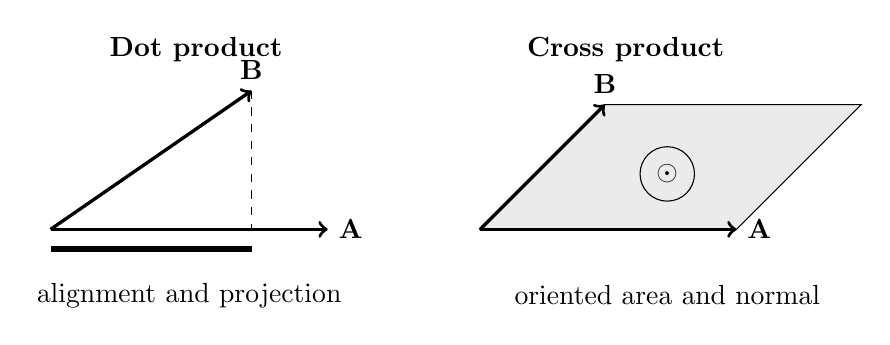
\begin{tikzpicture}[scale=0.88]
  \begin{scope}
    \node[font=\bfseries] at (2.4,3.1) {Dot product};
    \draw[->,very thick] (0.3,0.5)--(4.3,0.5) node[right] {$\mathbf A$};
    \draw[->,very thick] (0.3,0.5)--(3.2,2.5) node[above] {$\mathbf B$};
    \draw[dashed] (3.2,2.5)--(3.2,0.5);
    \draw[line width=2pt] (0.3,0.22)--(3.2,0.22);
    \node at (2.3,-0.45) {alignment and projection};
  \end{scope}
  \begin{scope}[xshift=6.2cm]
    \node[font=\bfseries] at (2.4,3.1) {Cross product};
    \fill[black!8] (0.3,0.5)--(4.0,0.5)--(5.8,2.3)--(2.1,2.3)--cycle;
    \draw (0.3,0.5)--(4.0,0.5)--(5.8,2.3)--(2.1,2.3)--cycle;
    \draw[->,very thick] (0.3,0.5)--(4.0,0.5) node[right] {$\mathbf A$};
    \draw[->,very thick] (0.3,0.5)--(2.1,2.3) node[above] {$\mathbf B$};
    \node[circle,draw] at (3.0,1.3) {$\odot$};
    \node at (3.0,-0.45) {oriented area and normal};
  \end{scope}
\end{tikzpicture}
\end{bookfigure}

\chapterformulaheading
\begin{formulasheetbox}
\begin{formulatable}
Vector expansion & $\mathbf v=\sum_i v^i\mathbf e_i$\\
Magnitude & $\lVert\mathbf v\rVert=\sqrt{\mathbf v\cdot\mathbf v}$\\
Unit vector & $\widehat{\mathbf v}=\mathbf v/\lVert\mathbf v\rVert$\\
Dot product & $\mathbf a\cdot\mathbf b=\lVert\mathbf a\rVert\lVert\mathbf b\rVert\cos\theta$\\
Cross product & $\lVert\mathbf a\times\mathbf b\rVert=\lVert\mathbf a\rVert\lVert\mathbf b\rVert\sin\theta$\\
Projection & $\operatorname{proj}_{\mathbf a}\mathbf v=(\mathbf v\cdot\mathbf a/\mathbf a\cdot\mathbf a)\mathbf a$\\
Linear independence & $\sum_i c_i\mathbf v_i=\mathbf0\Rightarrow c_i=0$ for all $i$\\
Eigenvector equation & $T\mathbf v=\lambda\mathbf v$\\
\end{formulatable}
\end{formulasheetbox}

\chapternotationheading
\begin{notationbox}
\begin{notationtable}
$\mathbf r$ & Position vector & m\\
$\mathbf a,\mathbf b,\mathbf v$ & General vectors & context dependent\\
$\mathbf e_i$ & Basis vector & usually dimensionless\\
$\widehat{\mathbf n}$ & Unit direction or unit normal & dimensionless\\
$\theta$ & Angle between vectors & rad\\
$T$ & Linear transformation & context dependent\\
$\lambda$ & Scalar or eigenvalue & context dependent\\
\end{notationtable}
\end{notationbox}

\begin{warningbox}
Do not identify a vector with one particular column of components. Components change under a change of basis; the vector itself does not. Likewise, a nonzero magnitude does not determine a direction, and a zero vector cannot be normalized.
\end{warningbox}

\chapteroutcomesheading
\begin{outcomesbox}
After studying this chapter, the reader should be able to:
\begin{itemize}
\item distinguish physical quantities from their coordinate representations;
\item compute vector sums, magnitudes, dot products, cross products, and projections;
\item interpret signs, directions, areas, and orthogonality physically;
\item test linear independence and construct coordinates in a basis;
\item recognize functions, matrices, and quantum states as vectors in suitable spaces;
\item explain why a change of basis changes components but not the represented object.
\end{itemize}
\end{outcomesbox}

\chapterlookaheadheading
\begin{lookingaheadbox}
Chapter~\ref{ch:differential-calculus} makes physical quantities vary continuously. Position becomes a function $\mathbf r(t)$; derivatives generate velocity and acceleration; and local linear approximation becomes the central tool connecting geometry with dynamics:
\[
\mathbf r(t)
\longrightarrow
\frac{d\mathbf r}{dt}
\longrightarrow
\frac{d^2\mathbf r}{dt^2}.
\]
The computational experiments in Section~\ref{sec:ch1-computational-companion} provide a numerical preview of this transition. The basis and projection ideas developed here will also reappear in gradients, fields, normal modes, and quantum measurement.
\end{lookingaheadbox}
